\documentclass[11pt]{article}

\usepackage[margin=1in]{geometry}
\usepackage{amsmath,amssymb}
\usepackage{booktabs}
\usepackage{graphicx}
\usepackage{caption}
\usepackage{hyperref}
\usepackage{xcolor}
\usepackage{enumitem}
\usepackage{tikz}
\usetikzlibrary{positioning,arrows.meta}
\hypersetup{colorlinks=true, linkcolor=blue!50!black, urlcolor=blue!50!black,
            citecolor=blue!50!black}

% Generated numbers. Every value the results section reports is defined here by
% scripts/make_exonaut_paper_assets.py from the row-level CSV. Nothing is typed.
% AUTO-GENERATED by scripts/make_exonaut_paper_assets.py from exonaut_main.csv
% Do not edit by hand. Regenerate instead.
\newcommand{\MainMissions}{750}
\newcommand{\MainConditions}{5}
\newcommand{\MainPlanners}{3}
\newcommand{\MainSeedsPerCondition}{50}
\newcommand{\MainCommit}{a5e5081728c8}
\newcommand{\MainSplitChecksum}{c9346c400ce5}
\newcommand{\MainMarsCommAdaptiveSuccess}{0.44}
\newcommand{\MainMarsCommAdaptiveScience}{0.156}
\newcommand{\MainMarsCommAdaptiveImmob}{2}
\newcommand{\MainMarsCommAdaptiveEnergyOut}{23}
\newcommand{\MainMarsCommAdaptiveInterventions}{8.1}
\newcommand{\MainMarsCommAdaptiveSlipEvents}{2.60}
\newcommand{\MainMarsCommAstarSuccess}{0.54}
\newcommand{\MainMarsCommAstarScience}{0.107}
\newcommand{\MainMarsCommAstarImmob}{3}
\newcommand{\MainMarsCommAstarEnergyOut}{19}
\newcommand{\MainMarsCommAstarInterventions}{6.8}
\newcommand{\MainMarsCommAstarSlipEvents}{2.34}
\newcommand{\MainMarsCommFixedSuccess}{0.28}
\newcommand{\MainMarsCommFixedScience}{0.200}
\newcommand{\MainMarsCommFixedImmob}{4}
\newcommand{\MainMarsCommFixedEnergyOut}{26}
\newcommand{\MainMarsCommFixedInterventions}{11.6}
\newcommand{\MainMarsCommFixedSlipEvents}{3.24}
\newcommand{\MainMarsFaultAdaptiveSuccess}{0.46}
\newcommand{\MainMarsFaultAdaptiveScience}{0.146}
\newcommand{\MainMarsFaultAdaptiveImmob}{8}
\newcommand{\MainMarsFaultAdaptiveEnergyOut}{17}
\newcommand{\MainMarsFaultAdaptiveInterventions}{66.8}
\newcommand{\MainMarsFaultAdaptiveSlipEvents}{3.44}
\newcommand{\MainMarsFaultAstarSuccess}{0.40}
\newcommand{\MainMarsFaultAstarScience}{0.074}
\newcommand{\MainMarsFaultAstarImmob}{9}
\newcommand{\MainMarsFaultAstarEnergyOut}{20}
\newcommand{\MainMarsFaultAstarInterventions}{48.5}
\newcommand{\MainMarsFaultAstarSlipEvents}{3.60}
\newcommand{\MainMarsFaultFixedSuccess}{0.26}
\newcommand{\MainMarsFaultFixedScience}{0.168}
\newcommand{\MainMarsFaultFixedImmob}{9}
\newcommand{\MainMarsFaultFixedEnergyOut}{24}
\newcommand{\MainMarsFaultFixedInterventions}{95.6}
\newcommand{\MainMarsFaultFixedSlipEvents}{4.42}
\newcommand{\MainMarsUncAdaptiveSuccess}{0.36}
\newcommand{\MainMarsUncAdaptiveScience}{0.132}
\newcommand{\MainMarsUncAdaptiveImmob}{7}
\newcommand{\MainMarsUncAdaptiveEnergyOut}{22}
\newcommand{\MainMarsUncAdaptiveInterventions}{88.7}
\newcommand{\MainMarsUncAdaptiveSlipEvents}{3.96}
\newcommand{\MainMarsUncAstarSuccess}{0.44}
\newcommand{\MainMarsUncAstarScience}{0.081}
\newcommand{\MainMarsUncAstarImmob}{8}
\newcommand{\MainMarsUncAstarEnergyOut}{20}
\newcommand{\MainMarsUncAstarInterventions}{45.3}
\newcommand{\MainMarsUncAstarSlipEvents}{3.00}
\newcommand{\MainMarsUncFixedSuccess}{0.22}
\newcommand{\MainMarsUncFixedScience}{0.162}
\newcommand{\MainMarsUncFixedImmob}{8}
\newcommand{\MainMarsUncFixedEnergyOut}{27}
\newcommand{\MainMarsUncFixedInterventions}{83.7}
\newcommand{\MainMarsUncFixedSlipEvents}{3.72}
\newcommand{\MainMarsOODAdaptiveSuccess}{0.34}
\newcommand{\MainMarsOODAdaptiveScience}{0.158}
\newcommand{\MainMarsOODAdaptiveImmob}{7}
\newcommand{\MainMarsOODAdaptiveEnergyOut}{20}
\newcommand{\MainMarsOODAdaptiveInterventions}{89.7}
\newcommand{\MainMarsOODAdaptiveSlipEvents}{4.00}
\newcommand{\MainMarsOODAstarSuccess}{0.48}
\newcommand{\MainMarsOODAstarScience}{0.101}
\newcommand{\MainMarsOODAstarImmob}{7}
\newcommand{\MainMarsOODAstarEnergyOut}{18}
\newcommand{\MainMarsOODAstarInterventions}{57.5}
\newcommand{\MainMarsOODAstarSlipEvents}{3.38}
\newcommand{\MainMarsOODFixedSuccess}{0.34}
\newcommand{\MainMarsOODFixedScience}{0.173}
\newcommand{\MainMarsOODFixedImmob}{6}
\newcommand{\MainMarsOODFixedEnergyOut}{21}
\newcommand{\MainMarsOODFixedInterventions}{102.8}
\newcommand{\MainMarsOODFixedSlipEvents}{4.14}
\newcommand{\MainMoonIDAdaptiveSuccess}{0.92}
\newcommand{\MainMoonIDAdaptiveScience}{0.829}
\newcommand{\MainMoonIDAdaptiveImmob}{0}
\newcommand{\MainMoonIDAdaptiveEnergyOut}{3}
\newcommand{\MainMoonIDAdaptiveInterventions}{20.1}
\newcommand{\MainMoonIDAdaptiveSlipEvents}{0.16}
\newcommand{\MainMoonIDAstarSuccess}{0.66}
\newcommand{\MainMoonIDAstarScience}{0.659}
\newcommand{\MainMoonIDAstarImmob}{0}
\newcommand{\MainMoonIDAstarEnergyOut}{12}
\newcommand{\MainMoonIDAstarInterventions}{29.6}
\newcommand{\MainMoonIDAstarSlipEvents}{0.12}
\newcommand{\MainMoonIDFixedSuccess}{0.90}
\newcommand{\MainMoonIDFixedScience}{0.788}
\newcommand{\MainMoonIDFixedImmob}{0}
\newcommand{\MainMoonIDFixedEnergyOut}{4}
\newcommand{\MainMoonIDFixedInterventions}{32.5}
\newcommand{\MainMoonIDFixedSlipEvents}{0.24}
\newcommand{\MainDeltaMarsCommScience}{-0.044}
\newcommand{\MainPMarsCommScience}{0.326}
\newcommand{\MainDeltaMarsCommSuccess}{+0.160}
\newcommand{\MainPMarsCommSuccess}{0.461}
\newcommand{\MainDeltaMarsFaultScience}{-0.022}
\newcommand{\MainPMarsFaultScience}{0.461}
\newcommand{\MainDeltaMarsFaultSuccess}{+0.200}
\newcommand{\MainPMarsFaultSuccess}{0.020}
\newcommand{\MainDeltaMarsUncScience}{-0.030}
\newcommand{\MainPMarsUncScience}{0.326}
\newcommand{\MainDeltaMarsUncSuccess}{+0.140}
\newcommand{\MainPMarsUncSuccess}{0.461}
\newcommand{\MainDeltaMarsOODScience}{-0.015}
\newcommand{\MainPMarsOODScience}{1.000}
\newcommand{\MainDeltaMarsOODSuccess}{+0.000}
\newcommand{\MainPMarsOODSuccess}{1.000}
\newcommand{\MainDeltaMoonIDScience}{+0.040}
\newcommand{\MainPMoonIDScience}{0.326}
\newcommand{\MainDeltaMoonIDSuccess}{+0.020}
\newcommand{\MainPMoonIDSuccess}{1.000}
\newcommand{\MainGapAdaptive}{0.670}
\newcommand{\MainGapAstar}{0.558}
\newcommand{\MainGapFixed}{0.615}

% Post-hoc audits (not in the analysis plan), generated by
% scripts/audit_confirmatory.py.
% AUTO-GENERATED by scripts/audit_confirmatory.py - post-hoc audits, not confirmatory
\newcommand{\AuditReproduced}{100\%}
\newcommand{\AuditFiredAdaptive}{16\%}
\newcommand{\AuditFiredFixed}{26\%}
\newcommand{\AuditFiredAstar}{10\%}
\newcommand{\AuditMedianSteps}{91}
\newcommand{\AuditHorizon}{800}
\newcommand{\AuditDiscordant}{10}
\newcommand{\AuditDiscordantBoth}{1}
\newcommand{\AuditDiscordantNone}{5}
\newcommand{\AuditDiscordantMixed}{4}
\newcommand{\AuditCoverageCommitted}{0.20}
\newcommand{\AuditCoverageCorrected}{0.85}
\newcommand{\AuditErrorCommitted}{0.060}
\newcommand{\AuditErrorCorrected}{0.017}
\newcommand{\AuditSdCommitted}{0.0089}
\newcommand{\AuditCalibrationMissions}{40}

% Development work for Study 2 (train and validation seeds only), generated by
% scripts/calibration_paper_assets.py and scripts/power_analysis.py.
% Provenance for every generated file: paper/PROVENANCE.yaml.
% AUTO-GENERATED by scripts/calibration_paper_assets.py from data/validation/calibration/.
% Train and validation seeds only. Not confirmatory.
\newcommand{\CalDiagNoMisclassMarsCovFifty}{0.31}
\newcommand{\CalDiagNoMisclassMarsCovEighty}{0.56}
\newcommand{\CalDiagNoMisclassMarsCovNinety}{0.65}
\newcommand{\CalDiagNoMisclassMarsCovNinetyFive}{0.74}
\newcommand{\CalDiagNoMisclassMarsCovNinetyFiveLo}{0.68}
\newcommand{\CalDiagNoMisclassMarsCovNinetyFiveHi}{0.78}
\newcommand{\CalDiagNoMisclassMarsMedianSd}{0.025}
\newcommand{\CalDiagNoMisclassMarsMedianError}{0.019}
\newcommand{\CalDiagNoMisclassMarsMissions}{100}
\newcommand{\CalDiagNoMisclassMoonCovFifty}{0.55}
\newcommand{\CalDiagNoMisclassMoonCovEighty}{0.88}
\newcommand{\CalDiagNoMisclassMoonCovNinety}{0.95}
\newcommand{\CalDiagNoMisclassMoonCovNinetyFive}{0.98}
\newcommand{\CalDiagNoMisclassMoonCovNinetyFiveLo}{0.96}
\newcommand{\CalDiagNoMisclassMoonCovNinetyFiveHi}{0.99}
\newcommand{\CalDiagNoMisclassMoonMedianSd}{0.014}
\newcommand{\CalDiagNoMisclassMoonMedianError}{0.009}
\newcommand{\CalDiagNoMisclassMoonMissions}{100}
\newcommand{\CalDiagTrueDispersionMarsCovFifty}{0.26}
\newcommand{\CalDiagTrueDispersionMarsCovEighty}{0.41}
\newcommand{\CalDiagTrueDispersionMarsCovNinety}{0.48}
\newcommand{\CalDiagTrueDispersionMarsCovNinetyFive}{0.52}
\newcommand{\CalDiagTrueDispersionMarsCovNinetyFiveLo}{0.48}
\newcommand{\CalDiagTrueDispersionMarsCovNinetyFiveHi}{0.55}
\newcommand{\CalDiagTrueDispersionMarsMedianSd}{0.026}
\newcommand{\CalDiagTrueDispersionMarsMedianError}{0.049}
\newcommand{\CalDiagTrueDispersionMarsMissions}{100}
\newcommand{\CalDiagTrueDispersionMoonCovFifty}{0.25}
\newcommand{\CalDiagTrueDispersionMoonCovEighty}{0.49}
\newcommand{\CalDiagTrueDispersionMoonCovNinety}{0.57}
\newcommand{\CalDiagTrueDispersionMoonCovNinetyFive}{0.64}
\newcommand{\CalDiagTrueDispersionMoonCovNinetyFiveLo}{0.58}
\newcommand{\CalDiagTrueDispersionMoonCovNinetyFiveHi}{0.68}
\newcommand{\CalDiagTrueDispersionMoonMedianSd}{0.015}
\newcommand{\CalDiagTrueDispersionMoonMedianError}{0.026}
\newcommand{\CalDiagTrueDispersionMoonMissions}{100}
\newcommand{\CalDiagTruePriorMeanMarsCovFifty}{0.28}
\newcommand{\CalDiagTruePriorMeanMarsCovEighty}{0.43}
\newcommand{\CalDiagTruePriorMeanMarsCovNinety}{0.51}
\newcommand{\CalDiagTruePriorMeanMarsCovNinetyFive}{0.57}
\newcommand{\CalDiagTruePriorMeanMarsCovNinetyFiveLo}{0.52}
\newcommand{\CalDiagTruePriorMeanMarsCovNinetyFiveHi}{0.63}
\newcommand{\CalDiagTruePriorMeanMarsMedianSd}{0.025}
\newcommand{\CalDiagTruePriorMeanMarsMedianError}{0.039}
\newcommand{\CalDiagTruePriorMeanMarsMissions}{100}
\newcommand{\CalDiagTruePriorMeanMoonCovFifty}{0.27}
\newcommand{\CalDiagTruePriorMeanMoonCovEighty}{0.48}
\newcommand{\CalDiagTruePriorMeanMoonCovNinety}{0.57}
\newcommand{\CalDiagTruePriorMeanMoonCovNinetyFive}{0.64}
\newcommand{\CalDiagTruePriorMeanMoonCovNinetyFiveLo}{0.58}
\newcommand{\CalDiagTruePriorMeanMoonCovNinetyFiveHi}{0.69}
\newcommand{\CalDiagTruePriorMeanMoonMedianSd}{0.016}
\newcommand{\CalDiagTruePriorMeanMoonMedianError}{0.024}
\newcommand{\CalDiagTruePriorMeanMoonMissions}{100}
\newcommand{\CalDiagBaseMarsCovFifty}{0.25}
\newcommand{\CalDiagBaseMarsCovEighty}{0.39}
\newcommand{\CalDiagBaseMarsCovNinety}{0.45}
\newcommand{\CalDiagBaseMarsCovNinetyFive}{0.50}
\newcommand{\CalDiagBaseMarsCovNinetyFiveLo}{0.46}
\newcommand{\CalDiagBaseMarsCovNinetyFiveHi}{0.53}
\newcommand{\CalDiagBaseMarsMedianSd}{0.025}
\newcommand{\CalDiagBaseMarsMedianError}{0.050}
\newcommand{\CalDiagBaseMarsMissions}{100}
\newcommand{\CalDiagBaseMoonCovFifty}{0.27}
\newcommand{\CalDiagBaseMoonCovEighty}{0.51}
\newcommand{\CalDiagBaseMoonCovNinety}{0.60}
\newcommand{\CalDiagBaseMoonCovNinetyFive}{0.68}
\newcommand{\CalDiagBaseMoonCovNinetyFiveLo}{0.65}
\newcommand{\CalDiagBaseMoonCovNinetyFiveHi}{0.71}
\newcommand{\CalDiagBaseMoonMedianSd}{0.019}
\newcommand{\CalDiagBaseMoonMedianError}{0.025}
\newcommand{\CalDiagBaseMoonMissions}{100}
\newcommand{\CalDiagNoMisclassMarsPredCovNinety}{0.74}
\newcommand{\CalDiagNoMisclassMarsSevereRate}{0.050}
\newcommand{\CalDiagNoMisclassMarsMeanPSevere}{0.021}
\newcommand{\CalDiagNoMisclassMarsBrier}{0.0429}
\newcommand{\CalDiagNoMisclassMoonPredCovNinety}{0.84}
\newcommand{\CalDiagNoMisclassMoonSevereRate}{0.001}
\newcommand{\CalDiagNoMisclassMoonMeanPSevere}{0.001}
\newcommand{\CalDiagNoMisclassMoonBrier}{0.0009}
\newcommand{\CalDiagTrueDispersionMarsPredCovNinety}{0.85}
\newcommand{\CalDiagTrueDispersionMarsSevereRate}{0.046}
\newcommand{\CalDiagTrueDispersionMarsMeanPSevere}{0.023}
\newcommand{\CalDiagTrueDispersionMarsBrier}{0.0386}
\newcommand{\CalDiagTrueDispersionMoonPredCovNinety}{0.84}
\newcommand{\CalDiagTrueDispersionMoonSevereRate}{0.001}
\newcommand{\CalDiagTrueDispersionMoonMeanPSevere}{0.001}
\newcommand{\CalDiagTrueDispersionMoonBrier}{0.0008}
\newcommand{\CalDiagTruePriorMeanMarsPredCovNinety}{0.73}
\newcommand{\CalDiagTruePriorMeanMarsSevereRate}{0.045}
\newcommand{\CalDiagTruePriorMeanMarsMeanPSevere}{0.031}
\newcommand{\CalDiagTruePriorMeanMarsBrier}{0.0366}
\newcommand{\CalDiagTruePriorMeanMoonPredCovNinety}{0.84}
\newcommand{\CalDiagTruePriorMeanMoonSevereRate}{0.001}
\newcommand{\CalDiagTruePriorMeanMoonMeanPSevere}{0.001}
\newcommand{\CalDiagTruePriorMeanMoonBrier}{0.0005}
\newcommand{\CalDiagBaseMarsPredCovNinety}{0.72}
\newcommand{\CalDiagBaseMarsSevereRate}{0.042}
\newcommand{\CalDiagBaseMarsMeanPSevere}{0.015}
\newcommand{\CalDiagBaseMarsBrier}{0.0371}
\newcommand{\CalDiagBaseMoonPredCovNinety}{0.83}
\newcommand{\CalDiagBaseMoonSevereRate}{0.001}
\newcommand{\CalDiagBaseMoonMeanPSevere}{0.001}
\newcommand{\CalDiagBaseMoonBrier}{0.0007}
\newcommand{\CalMisclassShareMars}{9.8}
\newcommand{\CalMisclassShareMoon}{10.3}
\newcommand{\CalScaleMTwoMars}{8.49}
\newcommand{\CalScaleMTwoMoon}{4.77}
\newcommand{\CalScaleMFourMars}{2.94}
\newcommand{\CalScaleMFourMoon}{1.00}
\newcommand{\CalEvaluated}{yes}
\newcommand{\CalMOneMarsCovFifty}{0.25}
\newcommand{\CalMOneMarsCovEighty}{0.41}
\newcommand{\CalMOneMarsCovNinety}{0.49}
\newcommand{\CalMOneMarsCovNinetyFive}{0.54}
\newcommand{\CalMOneMarsCovNinetyFiveLo}{0.49}
\newcommand{\CalMOneMarsCovNinetyFiveHi}{0.57}
\newcommand{\CalMOneMarsMedianSd}{0.025}
\newcommand{\CalMOneMarsMedianError}{0.036}
\newcommand{\CalMOneMarsMissions}{100}
\newcommand{\CalMOneMoonCovFifty}{0.28}
\newcommand{\CalMOneMoonCovEighty}{0.47}
\newcommand{\CalMOneMoonCovNinety}{0.55}
\newcommand{\CalMOneMoonCovNinetyFive}{0.65}
\newcommand{\CalMOneMoonCovNinetyFiveLo}{0.57}
\newcommand{\CalMOneMoonCovNinetyFiveHi}{0.71}
\newcommand{\CalMOneMoonMedianSd}{0.015}
\newcommand{\CalMOneMoonMedianError}{0.029}
\newcommand{\CalMOneMoonMissions}{100}
\newcommand{\CalMTwoAMarsCovFifty}{0.69}
\newcommand{\CalMTwoAMarsCovEighty}{0.88}
\newcommand{\CalMTwoAMarsCovNinety}{0.92}
\newcommand{\CalMTwoAMarsCovNinetyFive}{0.95}
\newcommand{\CalMTwoAMarsCovNinetyFiveLo}{0.91}
\newcommand{\CalMTwoAMarsCovNinetyFiveHi}{0.97}
\newcommand{\CalMTwoAMarsMedianSd}{0.121}
\newcommand{\CalMTwoAMarsMedianError}{0.039}
\newcommand{\CalMTwoAMarsMissions}{100}
\newcommand{\CalMTwoAMoonCovFifty}{0.83}
\newcommand{\CalMTwoAMoonCovEighty}{0.93}
\newcommand{\CalMTwoAMoonCovNinety}{0.95}
\newcommand{\CalMTwoAMoonCovNinetyFive}{0.97}
\newcommand{\CalMTwoAMoonCovNinetyFiveLo}{0.95}
\newcommand{\CalMTwoAMoonCovNinetyFiveHi}{0.98}
\newcommand{\CalMTwoAMoonMedianSd}{0.084}
\newcommand{\CalMTwoAMoonMedianError}{0.024}
\newcommand{\CalMTwoAMoonMissions}{100}
\newcommand{\CalMTwoBMarsCovFifty}{0.88}
\newcommand{\CalMTwoBMarsCovEighty}{0.97}
\newcommand{\CalMTwoBMarsCovNinety}{0.97}
\newcommand{\CalMTwoBMarsCovNinetyFive}{0.98}
\newcommand{\CalMTwoBMarsCovNinetyFiveLo}{0.96}
\newcommand{\CalMTwoBMarsCovNinetyFiveHi}{0.99}
\newcommand{\CalMTwoBMarsMedianSd}{0.215}
\newcommand{\CalMTwoBMarsMedianError}{0.037}
\newcommand{\CalMTwoBMarsMissions}{100}
\newcommand{\CalMTwoBMoonCovFifty}{0.92}
\newcommand{\CalMTwoBMoonCovEighty}{0.97}
\newcommand{\CalMTwoBMoonCovNinety}{0.99}
\newcommand{\CalMTwoBMoonCovNinetyFive}{1.00}
\newcommand{\CalMTwoBMoonCovNinetyFiveLo}{0.99}
\newcommand{\CalMTwoBMoonCovNinetyFiveHi}{1.00}
\newcommand{\CalMTwoBMoonMedianSd}{0.140}
\newcommand{\CalMTwoBMoonMedianError}{0.025}
\newcommand{\CalMTwoBMoonMissions}{100}
\newcommand{\CalMThreeMarsCovFifty}{0.36}
\newcommand{\CalMThreeMarsCovEighty}{0.57}
\newcommand{\CalMThreeMarsCovNinety}{0.66}
\newcommand{\CalMThreeMarsCovNinetyFive}{0.72}
\newcommand{\CalMThreeMarsCovNinetyFiveLo}{0.68}
\newcommand{\CalMThreeMarsCovNinetyFiveHi}{0.76}
\newcommand{\CalMThreeMarsMedianSd}{0.029}
\newcommand{\CalMThreeMarsMedianError}{0.020}
\newcommand{\CalMThreeMarsMissions}{100}
\newcommand{\CalMThreeMoonCovFifty}{0.55}
\newcommand{\CalMThreeMoonCovEighty}{0.83}
\newcommand{\CalMThreeMoonCovNinety}{0.92}
\newcommand{\CalMThreeMoonCovNinetyFive}{0.96}
\newcommand{\CalMThreeMoonCovNinetyFiveLo}{0.94}
\newcommand{\CalMThreeMoonCovNinetyFiveHi}{0.98}
\newcommand{\CalMThreeMoonMedianSd}{0.016}
\newcommand{\CalMThreeMoonMedianError}{0.008}
\newcommand{\CalMThreeMoonMissions}{100}
\newcommand{\CalMFourAMarsCovFifty}{0.36}
\newcommand{\CalMFourAMarsCovEighty}{0.57}
\newcommand{\CalMFourAMarsCovNinety}{0.66}
\newcommand{\CalMFourAMarsCovNinetyFive}{0.72}
\newcommand{\CalMFourAMarsCovNinetyFiveLo}{0.68}
\newcommand{\CalMFourAMarsCovNinetyFiveHi}{0.76}
\newcommand{\CalMFourAMarsMedianSd}{0.029}
\newcommand{\CalMFourAMarsMedianError}{0.020}
\newcommand{\CalMFourAMarsMissions}{100}
\newcommand{\CalMFourAMoonCovFifty}{0.55}
\newcommand{\CalMFourAMoonCovEighty}{0.83}
\newcommand{\CalMFourAMoonCovNinety}{0.92}
\newcommand{\CalMFourAMoonCovNinetyFive}{0.96}
\newcommand{\CalMFourAMoonCovNinetyFiveLo}{0.94}
\newcommand{\CalMFourAMoonCovNinetyFiveHi}{0.98}
\newcommand{\CalMFourAMoonMedianSd}{0.016}
\newcommand{\CalMFourAMoonMedianError}{0.008}
\newcommand{\CalMFourAMoonMissions}{100}
\newcommand{\CalMFourBMarsCovFifty}{0.72}
\newcommand{\CalMFourBMarsCovEighty}{0.90}
\newcommand{\CalMFourBMarsCovNinety}{0.95}
\newcommand{\CalMFourBMarsCovNinetyFive}{0.98}
\newcommand{\CalMFourBMarsCovNinetyFiveLo}{0.97}
\newcommand{\CalMFourBMarsCovNinetyFiveHi}{0.99}
\newcommand{\CalMFourBMarsMedianSd}{0.084}
\newcommand{\CalMFourBMarsMedianError}{0.019}
\newcommand{\CalMFourBMarsMissions}{100}
\newcommand{\CalMFourBMoonCovFifty}{0.94}
\newcommand{\CalMFourBMoonCovEighty}{1.00}
\newcommand{\CalMFourBMoonCovNinety}{1.00}
\newcommand{\CalMFourBMoonCovNinetyFive}{1.00}
\newcommand{\CalMFourBMoonCovNinetyFiveLo}{1.00}
\newcommand{\CalMFourBMoonCovNinetyFiveHi}{1.00}
\newcommand{\CalMFourBMoonMedianSd}{0.049}
\newcommand{\CalMFourBMoonMedianError}{0.010}
\newcommand{\CalMFourBMoonMissions}{100}
\newcommand{\CalMOneMarsPredCovNinety}{0.73}
\newcommand{\CalMOneMarsSevereRate}{0.036}
\newcommand{\CalMOneMarsMeanPSevere}{0.013}
\newcommand{\CalMOneMarsBrier}{0.0315}
\newcommand{\CalMOneMoonPredCovNinety}{0.83}
\newcommand{\CalMOneMoonSevereRate}{0.001}
\newcommand{\CalMOneMoonMeanPSevere}{0.001}
\newcommand{\CalMOneMoonBrier}{0.0010}
\newcommand{\CalMTwoAMarsPredCovNinety}{0.84}
\newcommand{\CalMTwoAMarsSevereRate}{0.049}
\newcommand{\CalMTwoAMarsMeanPSevere}{0.034}
\newcommand{\CalMTwoAMarsBrier}{0.0386}
\newcommand{\CalMTwoAMoonPredCovNinety}{0.93}
\newcommand{\CalMTwoAMoonSevereRate}{0.001}
\newcommand{\CalMTwoAMoonMeanPSevere}{0.007}
\newcommand{\CalMTwoAMoonBrier}{0.0011}
\newcommand{\CalMTwoBMarsPredCovNinety}{0.93}
\newcommand{\CalMTwoBMarsSevereRate}{0.045}
\newcommand{\CalMTwoBMarsMeanPSevere}{0.054}
\newcommand{\CalMTwoBMarsBrier}{0.0362}
\newcommand{\CalMTwoBMoonPredCovNinety}{0.97}
\newcommand{\CalMTwoBMoonSevereRate}{0.000}
\newcommand{\CalMTwoBMoonMeanPSevere}{0.016}
\newcommand{\CalMTwoBMoonBrier}{0.0029}
\newcommand{\CalMThreeMarsPredCovNinety}{0.73}
\newcommand{\CalMThreeMarsSevereRate}{0.038}
\newcommand{\CalMThreeMarsMeanPSevere}{0.016}
\newcommand{\CalMThreeMarsBrier}{0.0329}
\newcommand{\CalMThreeMoonPredCovNinety}{0.84}
\newcommand{\CalMThreeMoonSevereRate}{0.001}
\newcommand{\CalMThreeMoonMeanPSevere}{0.002}
\newcommand{\CalMThreeMoonBrier}{0.0010}
\newcommand{\CalMFourAMarsPredCovNinety}{0.73}
\newcommand{\CalMFourAMarsSevereRate}{0.038}
\newcommand{\CalMFourAMarsMeanPSevere}{0.016}
\newcommand{\CalMFourAMarsBrier}{0.0329}
\newcommand{\CalMFourAMoonPredCovNinety}{0.84}
\newcommand{\CalMFourAMoonSevereRate}{0.001}
\newcommand{\CalMFourAMoonMeanPSevere}{0.002}
\newcommand{\CalMFourAMoonBrier}{0.0010}
\newcommand{\CalMFourBMarsPredCovNinety}{0.81}
\newcommand{\CalMFourBMarsSevereRate}{0.037}
\newcommand{\CalMFourBMarsMeanPSevere}{0.021}
\newcommand{\CalMFourBMarsBrier}{0.0309}
\newcommand{\CalMFourBMoonPredCovNinety}{0.90}
\newcommand{\CalMFourBMoonSevereRate}{0.001}
\newcommand{\CalMFourBMoonMeanPSevere}{0.004}
\newcommand{\CalMFourBMoonBrier}{0.0010}
\newcommand{\CalStatus}{NOT ACCEPTED}
\newcommand{\CalSelected}{none}
\newcommand{\CalBestAvailable}{M2a}
\newcommand{\CalAcceptedCount}{0}
\newcommand{\CalMOneMarsBedrockCov}{0.27}
\newcommand{\CalMOneMarsFinesCov}{0.15}
\newcommand{\CalMOneMoonBedrockCov}{0.18}
\newcommand{\CalMOneMoonFinesCov}{0.68}
\newcommand{\CalMThreeMarsBedrockCov}{0.89}
\newcommand{\CalMThreeMarsFinesCov}{0.27}
\newcommand{\CalMThreeMoonBedrockCov}{0.89}
\newcommand{\CalMThreeMoonFinesCov}{0.96}

% AUTO-GENERATED by scripts/power_analysis.py from validation missions. Not confirmatory.
\newcommand{\PowAlpha}{0.05}
\newcommand{\PowTarget}{0.90}
\newcommand{\PowMinEffect}{0.10}
\newcommand{\PowPool}{1000}
\newcommand{\PowMThreeValSeeds}{200}
\newcommand{\PowMThreeMarsSuccessAdaptive}{0.575}
\newcommand{\PowMThreeMarsSuccessFixed}{0.505}
\newcommand{\PowMThreeMarsOnlyAdaptive}{24}
\newcommand{\PowMThreeMarsOnlyFixed}{10}
\newcommand{\PowMThreeMarsPsiHat}{0.170}
\newcommand{\PowMThreeMarsPsiUpper}{0.207}
\newcommand{\PowMThreeMarsDeltaHat}{+0.070}
\newcommand{\PowMThreeMoonSuccessAdaptive}{0.950}
\newcommand{\PowMThreeMoonSuccessFixed}{0.955}
\newcommand{\PowMThreeRecommendedN}{230}
\newcommand{\PowMThreeAtNExact}{0.912}
\newcommand{\PowMThreeAtNSimulated}{0.915}
\newcommand{\PowMThreeAtNPsiHat}{0.959}
\newcommand{\PowMThreeSciSd}{0.064}
\newcommand{\PowMThreeSciDetectable}{0.012}
\newcommand{\PowMTwoAValSeeds}{200}
\newcommand{\PowMTwoAMarsSuccessAdaptive}{0.570}
\newcommand{\PowMTwoAMarsSuccessFixed}{0.560}
\newcommand{\PowMTwoAMarsOnlyAdaptive}{21}
\newcommand{\PowMTwoAMarsOnlyFixed}{19}
\newcommand{\PowMTwoAMarsPsiHat}{0.200}
\newcommand{\PowMTwoAMarsPsiUpper}{0.239}
\newcommand{\PowMTwoAMarsDeltaHat}{+0.010}
\newcommand{\PowMTwoAMoonSuccessAdaptive}{0.965}
\newcommand{\PowMTwoAMoonSuccessFixed}{0.955}
\newcommand{\PowMTwoARecommendedN}{260}
\newcommand{\PowMTwoAAtNExact}{0.903}
\newcommand{\PowMTwoAAtNSimulated}{0.901}
\newcommand{\PowMTwoAAtNPsiHat}{0.950}
\newcommand{\PowMTwoASciSd}{0.072}
\newcommand{\PowMTwoASciDetectable}{0.013}


\title{\textbf{Adaptive Risk-Aware Autonomy for Robotic Exploration of\\
Uncertain Extraterrestrial Terrain}}
\author{Viraat Chauhan}
\date{\today}

\begin{document}
\maketitle

\begin{abstract}
\noindent
A planetary rover cannot be driven in real time from Earth, so it must decide
for itself which ground is safe enough to cross. Those decisions rest on a
terrain model built before launch, from whatever experience was available at
the time. This work asks what happens when that model is wrong --- when the
robot arrives somewhere whose ground does not behave the way its model says
--- and whether a robot that revises its model from its own driving survives
better than one that does not.

We build a controlled 2.5-D autonomy testbed in which a single solar-powered
rover must visit science targets and return to its lander before its energy
runs out, on terrain where wheel slip is stochastic, sensing is noisy and
range-limited, and sustained slip ends the mission by embedding the vehicle.
Three planners are compared on identical terrain: distance-only \mbox{A*}, a
fixed risk-aware planner, and an otherwise identical planner whose mobility
model is updated online from measured slip. The three differ only in their
objective and in whether that objective's inputs are revised, so a measured
difference is attributable to the decision rule rather than to a different
search implementation.

The central experiment is a domain shift. Every planner carries a mobility
prior calibrated on lunar terrain and is then evaluated on Martian terrain,
where the same terrain-class vocabulary carries substantially different slip
statistics. Across \MainMissions{} missions on frozen, held-out seeds, we
report the effect of online adaptation on mission success and science return,
and the generalization gap between in-distribution and out-of-distribution
performance.

The paper reports two studies. \emph{Study~1} is complete: a confirmatory run
on engine profile v1, reported with its pre-specified tests. An audit after it
found simulator and learner defects that change what several of its conditions
measured; those findings, their fixes, and a calibration audit of the terrain
learner on development data are reported as such. \emph{Study~2} is planned and
not yet executed: its question, hypotheses, sample-size analysis and seed
protocol are given, and it reports no results.

This is a simulation study of decision-making, not a validated model of any
flight vehicle or landing site. Section~\ref{sec:limitations} states plainly
what the model does and does not represent.
\end{abstract}

\section{Introduction}

Round-trip light time to Mars runs from roughly eight to forty minutes, and
contact windows are intermittent. A surface robot therefore cannot be
joysticked around a hazard; by the time an operator sees a problem, the
problem has already happened. Autonomy on planetary rovers exists for this
reason, and the quality of that autonomy is measured by what the robot does
when nobody can help it.

The failure mode that actually strands planetary rovers is not driving off a
cliff. It is sinking. A rover crossing ground that looks benign can lose
traction in loose material, dig itself in, and become permanently immobile.
NASA's \emph{Spirit} ended its driving mission this way in 2009, embedded in
soft soil~\cite{nasa_spirit}. What makes this failure mode interesting for autonomy research is
that it is invisible to geometry: the ground that traps a rover is often flat.
Detecting it requires a model of how terrain \emph{behaves}, not how it
\emph{looks}, and the only direct measurement of behaviour is slip observed
while driving on it.

That creates an asymmetry this paper is built around. Geometry --- slope,
roughness, obstacles --- can be sensed at a distance from imagery. Mobility
can only be measured by committing the vehicle to the ground. A robot
therefore plans long routes using a terrain model it cannot verify in advance,
and the model it starts with was calibrated somewhere else.

\paragraph{Research question.}
Does a planetary robot that continuously updates its terrain-mobility model
from its own driving make safer and more productive decisions than one using a
fixed model, when the terrain it encounters does not match the model it was
given?

\paragraph{Study 1 hypotheses.}
Stated before the Study~1 confirmatory data were generated (see
\texttt{docs/PREREGISTRATION.md}):
\begin{description}[leftmargin=2.2em,style=nextline]
  \item[H1] On in-distribution terrain, where the prior is already correct,
  adaptation neither helps nor harms: the adaptive and fixed planners perform
  equivalently.
  \item[H2] On out-of-distribution terrain, the adaptive planner returns a
  higher paired science fraction than the fixed planner.
  \item[H3] Under increased slip dispersion and injected faults, the adaptive
  planner achieves a higher mission-success rate and fewer severe-slip events.
  \item[H4] Intervention delay reduces productivity for all planners, and most
  for those that request more interventions.
\end{description}

\paragraph{What is and is not claimed as novel.}
Risk-aware planetary path planning, learned traversability, uncertainty-aware
terrain models and energy-constrained planning all exist in the literature and
are cited in Section~\ref{sec:related}. This work does not claim to invent any
of them. What it contributes is a controlled measurement: holding the search
algorithm, the cost function, the mission logic and the terrain fixed, and
changing \emph{only} whether the mobility model is revised online, in order to
isolate what that single mechanism is worth under a realistic domain shift.

\paragraph{Structure.}
Sections~\ref{sec:model}--\ref{sec:autonomy} describe the simulator and the
autonomy stack. Section~\ref{sec:study1} reports Study~1 as run. Section~\ref{sec:audit}
reports what was found after it --- simulator defects, their effect on
Study~1, and a calibration audit of the terrain learner --- and
Section~\ref{sec:study2} describes Study~2, which has not been run.

\section{Related work}
\label{sec:related}

Slip has long been treated as the operative traversability signal for Mars
rovers rather than slope alone; Angelova et al.~\cite{angelova2006slip} learned to predict slip from
terrain appearance, and Helmick et al.~\cite{helmick2007terrain} built
terrain-adaptive navigation around slip-aware models. More recent work makes the uncertainty explicit
rather than producing a single traversability score: Endo et al.~\cite{endo2023riskaware} fuse
probabilistic traversability predictions for risk-aware planning on
heterogeneous terrain, and extend this with test-time
adaptation~\cite{endo2024deepprob} so that a traversability model can be
corrected during deployment. Sanchez-Ibanez et al.~\cite{sanchez2022riskaware}
address a complementary risk, planning under localization uncertainty for
space exploration rovers.

The distinction this paper draws --- between uncertainty that more driving can
reduce and variability that it cannot --- follows the same motivation as that
line of work. Our contribution is not a better traversability model but a
controlled comparison of what online correction of such a model is worth when
the deployment environment differs from the calibration environment.

\section{Simulation model}
\label{sec:model}

\subsection{Scope}

The simulator is a controlled testbed for comparing decision rules. It is not
a validated dynamics model of a specific rover, and its absolute outputs are
properties of the model rather than predictions of on-surface performance. Its
purpose is to expose different planners to \emph{identical} stochastic worlds
so that differences between them are attributable to their decisions.

\subsection{Terrain}

Terrain is a $N \times N$ grid with an elevation field $z(x)$, from which slope
$\theta(x)$ is the gradient magnitude in degrees. Each cell carries a terrain
class $k(x)$ from a five-member vocabulary shared by both bodies: smooth
regolith, rocky, loose fines, bedrock, and rim talus. Each cell also carries a
roughness value, an illumination fraction $I(x) \in [0,1]$, and a hazard flag.

Crucially, the class \emph{vocabulary} is shared across bodies while the class
\emph{parameters} are not. Each body assigns every class a true mean slip
$\mu_k$, dispersion $\sigma_k$, and locomotion multiplier $m_k$. This is the
mechanism of the domain shift: a robot arriving at a new body recognizes the
same terrain categories but the statistics behind them have changed.

\subsection{Mobility and embedding}

When the robot commands a move into cell $x$, the realized slip fraction is

\begin{equation}
  s \sim \mathcal{N}\!\left(\mu_{k(x)} + \beta\,\theta(x) + b,\; \sigma_{k(x)}^2\right),
  \qquad s \in [0, 0.995],
  \label{eq:slip}
\end{equation}

with $\beta = 0.01$ per degree, representing traction lost on grades, and $b$ a
bias introduced by wheel-damage faults. A step is \emph{severe} when
$s \ge \tau$ with $\tau = 0.80$: the wheels turn but the robot does not
advance. After $L = 3$ consecutive severe steps the robot is permanently
embedded and the mission ends. This is the model's representation of the
Spirit-style loss mode, and it is the only failure with no recovery.

\subsection{Energy}

Energy to traverse a cell is

\begin{equation}
  E(x) \;=\; \frac{E_0 \, d \, m_{k(x)} \,\bigl(1 + \gamma\,\theta(x)\bigr)}
                  {\max(1 - s,\; \epsilon)}
             \cdot \frac{g}{g_{\mathrm{ref}}} \cdot \frac{1}{\eta_m},
  \label{eq:energy}
\end{equation}

with $d$ the distance in cells, $\gamma = 0.035$ per degree,
$\epsilon = 0.08$, $g$ the body's gravity against a lunar reference
$g_{\mathrm{ref}} = 1.62~\mathrm{m/s^2}$, and $\eta_m$ a motor-efficiency
factor degraded by faults. The slip term sits in the denominator because
slipping wheels still consume power while delivering less ground: at slip $s$,
covering the same distance costs roughly $1/(1-s)$ times as much.

Equation~\ref{eq:energy} is the reason a mobility error is also an energy
error, and it is the mechanism behind the results in
Section~\ref{sec:results}. A robot that underestimates slip underestimates the
cost of every route it considers.

Solar income per timestep is $\rho\, I(x)\, \eta_s$, with $\rho$ the nominal
harvest rate and $\eta_s$ an efficiency degraded by dust faults. Battery
capacity is scaled by $g/g_{\mathrm{ref}}$, representing a vehicle whose power
system is sized for the body it was built for; what transfers between bodies
in this study is the autonomy, not the hardware.

\subsection{Sensing}

The robot never reads ground truth. Within a sensing radius it receives noisy
estimates of slope, roughness, illumination, terrain class and hazard status,
with noise growing linearly in range. Terrain class is misclassified with a
range-dependent probability. Slip, by contrast, is measured directly and
without class ambiguity --- but only for the single cell just driven.

\section{Autonomy stack}
\label{sec:autonomy}

Figure~\ref{fig:flow} shows how information moves through the stack. The
rover senses a disc around itself, which grows its map of observed cells; its
belief about slip combines those observations with the class prior and, for
the adaptive planner only, with slip measured while driving; risk is computed
from that belief; and the mission manager chooses on risk. Belief
\emph{error}, the difference between belief and simulator truth, appears in
the figure only as an evaluation branch: the rover never has truth, so error
is something this study measures about the rover, not something the rover
uses.

\begin{figure}[t]
\centering
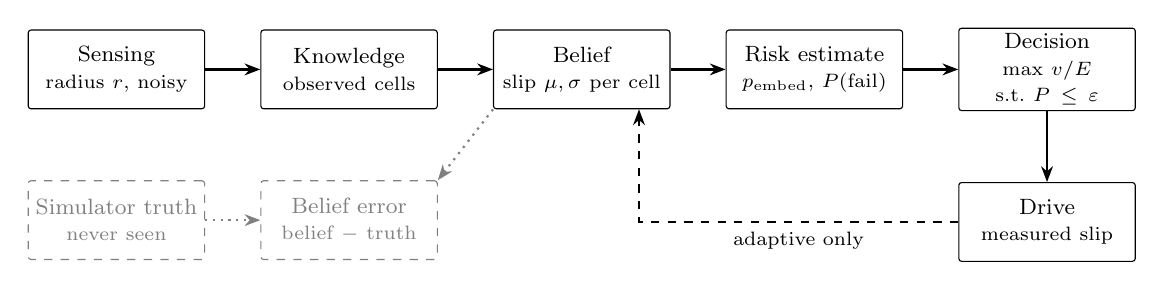
\begin{tikzpicture}[
  node distance=5mm and 7mm,
  box/.style={draw, rounded corners=1pt, align=center, font=\footnotesize,
              minimum height=10mm, text width=21mm, inner sep=2pt},
  eval/.style={box, dashed, draw=gray, text=gray},
  arr/.style={-{Stealth[length=2mm]}, thick},
]
\node[box] (sense) {Sensing\\ {\scriptsize radius $r$, noisy}};
\node[box, right=of sense] (know) {Knowledge\\ {\scriptsize observed cells}};
\node[box, right=of know] (belief) {Belief\\ {\scriptsize slip $\mu,\sigma$ per cell}};
\node[box, right=of belief] (risk) {Risk estimate\\ {\scriptsize $p_\text{embed}$, $P(\text{fail})$}};
\node[box, right=of risk] (plan) {Decision\\ {\scriptsize max $v/E$ s.t.\ $P\le\varepsilon$}};
\node[box, below=9mm of plan] (act) {Drive\\ {\scriptsize measured slip}};
\node[eval, below=9mm of know] (err) {Belief error\\ {\scriptsize belief $-$ truth}};
\node[eval, left=of err] (truth) {Simulator truth\\ {\scriptsize never seen}};
\draw[arr] (sense) -- (know);
\draw[arr] (know) -- (belief);
\draw[arr] (belief) -- (risk);
\draw[arr] (risk) -- (plan);
\draw[arr] (plan) -- (act);
\draw[arr, dashed] (act.west) -- node[below, font=\scriptsize] {adaptive only}
  ([xshift=-4mm]belief.south east |- act.west) -- ([xshift=-4mm]belief.south east);
\draw[arr, gray, dotted] (belief.south west) -- (err.north east);
\draw[arr, gray, dotted] (truth) -- (err);
\end{tikzpicture}
\caption{Information flow in the autonomy stack. Solid boxes are what the rover
computes and acts on. Dashed grey boxes are evaluation quantities available to
the study but not to the rover; belief error explains decisions after the fact
and is not an input to them. The dashed arrow (measured slip revising belief)
exists for the adaptive planner only.}
\label{fig:flow}
\end{figure}

\subsection{World model}

The robot maintains a belief, not the terrain. Per cell it stores the most
recent close-range geometric estimate. Per terrain class it stores a posterior
over mean slip, updated from driven experience by a Normal--Normal conjugate
model: with prior mean $m_0$, prior variance $t_0^2$, observation variance
$\sigma_o^2$ and $n$ measurements of sample mean $\bar{s}$,

\begin{equation}
  \lambda = \frac{1}{t_0^2} + \frac{n}{\sigma_o^2},
  \qquad
  m_n = \frac{1}{\lambda}\left(\frac{m_0}{t_0^2} + \frac{n \bar{s}}{\sigma_o^2}\right),
  \qquad
  t_n^2 = \frac{1}{\lambda}.
  \label{eq:conjugate}
\end{equation}

The posterior is recomputed from the prior and the full sample each time, so
it does not depend on update order.

\paragraph{Generalizing to unseen ground.}
Routes are composed mostly of cells the robot has never observed, so what it
believes about \emph{unknown} terrain determines almost every plan. For an
unobserved cell the class is unknown, and the expected slip is the current
class beliefs marginalized over the class mix $\pi_k$ actually encountered so
far:

\begin{equation}
  \hat{s}_{\mathrm{unk}} \;=\; \sum_k \pi_k \, m_n^{(k)}.
  \label{eq:unknown}
\end{equation}

This is what allows learning to transfer: measuring that the local drift sand
is treacherous raises the robot's estimate for ground it has not yet reached.
A fixed constant in place of Equation~\ref{eq:unknown} would confine every
lesson to cells already visited and, because routes are mostly unvisited
cells, would prevent adaptation from affecting any planning decision at all.

\paragraph{Two kinds of uncertainty.}
For unobserved cells the epistemic term combines the spread \emph{between}
class means with the uncertainty \emph{within} each:

\begin{equation}
  \sigma_{\mathrm{epi}}^2 = \underbrace{\sum_k \pi_k \bigl(m_n^{(k)} - \hat{s}_{\mathrm{unk}}\bigr)^2}_{\text{between classes}}
  \;+\; \underbrace{\sum_k \pi_k \, t_n^{2\,(k)}}_{\text{within class}},
  \qquad
  \sigma_{\mathrm{tot}}^2 = \sigma_{\mathrm{epi}}^2 + \sigma_{\mathrm{ale}}^2 .
  \label{eq:uncertainty}
\end{equation}

The separation matters: $\sigma_{\mathrm{epi}}$ is reducible by driving,
whereas $\sigma_{\mathrm{ale}}$ is the terrain's own variability and is not. A
planner that cannot tell them apart cannot distinguish ground that is
dangerous from ground that is merely unvisited.

\subsection{Risk}

Under the belief that slip at $x$ is $\mathcal{N}(\hat{s}, \sigma_{\mathrm{tot}}^2)$,
the probability of a severe step and of embedding are

\begin{equation}
  p_{\mathrm{sev}}(x) = 1 - \Phi\!\left(\frac{\tau - \hat{s}(x)}{\sigma_{\mathrm{tot}}(x)}\right),
  \qquad
  p_{\mathrm{emb}}(x) = p_{\mathrm{sev}}(x)^{L}.
  \label{eq:embed}
\end{equation}

Treating consecutive steps as independent \emph{understates} risk in
homogeneous terrain, where severe slip is spatially correlated and runs are
more likely than independence implies. The approximation is applied identically
to every planner and so cannot favour one.

A believed hazard is not by itself mission-ending: the robot's onboard
geometric check refuses such a command and replans. It enters the risk only
through the residual probability $\kappa = 0.005$ that the check misses it:

\begin{equation}
  R(x) \;=\; 1 - \bigl(1 - p_{\mathrm{emb}}(x)\bigr)\bigl(1 - \kappa\, p_{\mathrm{haz}}(x)\bigr),
  \qquad
  R(\pi) \;=\; 1 - \prod_{x \in \pi}\bigl(1 - R(x)\bigr).
  \label{eq:risk}
\end{equation}

Energy risk is evaluated against the usable budget, treating required energy as
normal with variance propagated from slip uncertainty by linearizing
Equation~\ref{eq:energy} about $\hat{s}$:

\begin{equation}
  \sigma_E^2 = \sum_{x \in \pi} \left(\frac{E(x)}{1 - \hat{s}(x)}\right)^{2}\!\sigma_{\mathrm{tot}}^2(x),
  \qquad
  P_{\mathrm{energy}} = \Pr\!\left[E_{\mathrm{req}} \ge B + S - R_{\mathrm{res}}\right],
  \label{eq:energyrisk}
\end{equation}

with $B$ the charge in hand, $S$ the solar income expected over the route, and
$R_{\mathrm{res}}$ a reserve held back as a fraction of capacity. Total mission
failure probability composes the two causes.

\subsection{Mission logic}

A mission is: start at the lander, visit science targets, return before the
energy runs out. The manager pursues the reachable target with the best
value-to-cost ratio whose round trip satisfies the risk budget
$P_{\mathrm{fail}} \le \varepsilon$, and otherwise returns home. Missions are
flown as sorties --- a target that does not fit on a low battery is
reconsidered after recharging, and written off only when the robot is home,
recharged, and still cannot reach it.

When no route is believed to exist, the robot must ask mission control. It
idles for the communication delay before receiving a relaxed instruction, and
each such episode is counted as a human intervention. An autonomy system that
succeeds only by asking for help frequently has not really succeeded, so
intervention count is reported alongside the outcome measures.

\subsection{The three planners}

All three run the same A* implementation over the same believed world and
differ only in the cost assigned to entering a cell.

\begin{description}[leftmargin=2.2em,style=nextline]
  \item[Distance-only A*] $J = d$. The control with no terrain model at all.
  \item[Fixed risk-aware A*] $J = w_d d + w_e E(x) + w_r R(x) + w_u \sigma_{\mathrm{epi}}(x)$,
  consulting the world model but never revising it.
  \item[Adaptive risk-aware A*] Identical objective and identical weights; the
  single difference is that measured slip is folded into the class belief via
  Equation~\ref{eq:conjugate}, so future plans use corrected estimates.
\end{description}

The adaptive planner is implemented as a subclass of the fixed planner that
overrides one method. The experimental treatment is therefore a single switch,
which is what makes the contrast interpretable.

\section{Study 1: design}
\label{sec:study1}

Study~1 ran on engine profile \emph{v1}. Its committed results are locked: a
SHA-256 of every artifact is recorded in \texttt{data/results/v1\_LOCK.json},
a test fails if any of them changes, and all \MainMissions{} missions were
re-run and reproduced exactly before the lock. Defects found later
(Section~\ref{sec:audit}) are reported, not repaired, in Study~1's results.

\subsection{Seed protocol}

Terrain seeds are partitioned into disjoint integer ranges --- train,
validation, test and out-of-distribution --- frozen to a checksummed file
before any result was generated. Priors are calibrated on train seeds only.
All tuning was performed on validation seeds. Test and OOD seeds informed no
design decision.

Eight seeds consumed by an earlier engineering pilot are permanently
quarantined and excluded from every confirmatory result; a regression test
asserts they cannot reappear. The confirmatory run used
\MainSeedsPerCondition{} seeds per condition from split checksum
\texttt{\MainSplitChecksum} at commit \texttt{\MainCommit}.

\subsection{Design}

\MainPlanners{} planners $\times$ \MainConditions{} conditions $\times$
\MainSeedsPerCondition{} seeds $=$ \MainMissions{} missions. Every planner is
evaluated on identical terrain within a condition, making this a randomized
block design in which terrain seed is the block.

Conditions: Moon in-distribution; Mars out-of-distribution; Mars with
$1.5\times$ slip dispersion; Mars with injected faults; and Mars with a
20-step intervention delay. Every condition uses a lunar-calibrated prior, so
the Martian conditions are genuine domain shifts.

\subsection{Analysis}

Because planners share terrain within a condition, all contrasts are paired.
Science fraction uses a paired $t$-test with a Wilcoxon signed-rank companion,
Cohen's $d_z$, and a 95\% confidence interval. Mission success is binary and
paired, so it uses McNemar's exact test~\cite{mcnemar1947}, which conditions on the
seeds where the two planners actually disagreed. Holm--Bonferroni correction~\cite{holm1979} is applied
across the prespecified primary family; secondary contrasts against the
distance-only control are corrected separately and never pooled with it.

We also report the generalization gap
$G = M_{\mathrm{in}} - M_{\mathrm{out}}$ per planner, a between-condition
descriptive quantity reported without a paired test because the conditions
draw from different seed splits.

\section{Study 1: results}
\label{sec:results}

All \MainMissions{} confirmatory missions completed without software error and
none were excluded. Results are reported for every outcome regardless of
significance, as the analysis plan requires.

\subsection{In-distribution: adaptation is neutral (H1 supported)}

On lunar terrain, where the prior is already correct, the adaptive and fixed
risk-aware planners are statistically indistinguishable: success
\MainMoonIDAdaptiveSuccess{} versus \MainMoonIDFixedSuccess{}
($\Delta = \MainDeltaMoonIDSuccess$, $p_{\mathrm{Holm}} = \MainPMoonIDSuccess$),
differing on only five of fifty seeds. This is what H1 predicted: when there is
nothing to learn, learning costs nothing.

Both risk-aware planners clearly beat the distance-only control here
(\MainMoonIDAstarSuccess{} success, \MainMoonIDAstarScience{} science
fraction), confirming that modelling terrain risk is worth doing when the
model is right.

\subsection{Out-of-distribution: H2 is not supported}

H2 predicted that adaptation would raise science fraction on Martian terrain.
It did not. In the baseline Martian condition the paired difference in science
fraction was $\MainDeltaMarsOODScience$
($p_{\mathrm{Holm}} = \MainPMarsOODScience$) --- a point estimate in the
\emph{opposite} direction to the hypothesis --- and mission success was exactly
tied, with each planner winning five of the ten seeds on which they differed.

We report this as a failure of the stated hypothesis rather than reframing it.
The validation-set estimate that motivated H2 (a success advantage of $+0.125$
to $+0.167$) did not replicate on held-out seeds. That divergence is itself the
argument for holding seeds back: a tuning-set effect of that size vanished
entirely under confirmatory evaluation.

\subsection{Degraded conditions: H3 not supported as stated}

The one contrast surviving Holm correction across the ten-member primary family
is mission success in the condition labelled ``hardware faults'', where the
adaptive planner succeeded more often than the fixed one
(\MainMarsFaultAdaptiveSuccess{} against \MainMarsFaultFixedSuccess{},
$\Delta = \MainDeltaMarsFaultSuccess$,
$p_{\mathrm{Holm}} = \MainPMarsFaultSuccess$), with all ten discordant seeds
favouring adaptation.

\textbf{This cannot be read as an effect of faults.} A post-hoc audit, which
was not part of the analysis plan, re-ran every mission in this condition. The
re-runs reproduced \AuditReproduced{} of the committed rows exactly. Faults are
scheduled uniformly across the \AuditHorizon-step horizon, but the median
mission in this condition ended after \AuditMedianSteps{} steps, so most
scheduled faults never fired. A fault actually occurred in only
\AuditFiredAdaptive{} of adaptive missions and \AuditFiredFixed{} of fixed
ones. Of the \AuditDiscordant{} discordant seeds behind the significant result,
a fault fired in both missions on \AuditDiscordantBoth{}, and in neither on
\AuditDiscordantNone{}.

So this condition mostly measured Martian missions without faults. It differs
from the plain Martian condition, where the same contrast was exactly zero,
chiefly through a shifted random stream (Section~\ref{sec:limitations}). The
most defensible reading is that this is sampling variation that survived
correction. We therefore do not claim support for H3. The other two degraded
conditions moved in the same direction without reaching corrected
significance: $\MainDeltaMarsUncSuccess$ under elevated slip dispersion
($p_{\mathrm{Holm}} = \MainPMarsUncSuccess$) and $\MainDeltaMarsCommSuccess$
under intervention delay ($p_{\mathrm{Holm}} = \MainPMarsCommSuccess$).

\subsection{A consistent, unconfirmed sign pattern}

Descriptively, in every Martian condition the adaptive planner's success rate is
at least the fixed planner's and its science fraction is slightly lower, and it
ends fewer missions in energy exhaustion. None of the science-fraction
differences survive correction, and the pattern was not a pre-specified test.

A mechanism is plausible. Locomotion cost carries a $1/(1-s)$ term
(Equation~\ref{eq:energy}), so a robot that raises its slip estimate raises its
estimate of every route's cost and turns back sooner. That trade would save
missions and cost science. But it is a hypothesis, not a finding, and a further
audit complicates it. The adaptive learner turned out to be badly
overconfident. On \AuditCalibrationMissions{} Martian validation missions, its
95\% intervals for class-mean slip contained the true value only
\AuditCoverageCommitted{} of the time, against 0.95 for a calibrated model. Its
median error was \AuditErrorCommitted{}, while it reported a median
uncertainty of just \AuditSdCommitted{}. The cause is that each slip reading is
treated as near-exact (Section~\ref{sec:limitations}). With the per-reading
variance set to the terrain's own dispersion, coverage rises only to
\AuditCoverageCorrected{} and median error falls to \AuditErrorCorrected{}. The
rest of the miscalibration comes from misclassification: the rover folds each
reading into the class it \emph{believes} it drove on, and some of those beliefs
are wrong. So
the method tested here adapts, but it adapts by over-reacting, and its effects
should not be read as the effects of a well-calibrated learner.

\subsection{An unanticipated result: the uninformed planner survives}

None of the hypotheses anticipated the clearest pattern in the Martian data.
Distance-only A*, which models no terrain risk whatsoever, achieved the
\emph{highest} mission-success rate of the three planners in three of the four
Martian conditions --- \MainMarsOODAstarSuccess{} against
\MainMarsOODFixedSuccess{} and \MainMarsOODAdaptiveSuccess{} in the baseline
OOD condition.

It also returned the least science (\MainMarsOODAstarScience{} against
\MainMarsOODFixedScience{} and \MainMarsOODAdaptiveScience{}). The
interpretation we favour, which the intervention counts support, is that
risk-averse routing on hostile terrain is expensive: the risk-aware planners
detour around suspect ground, and on Mars almost all ground is suspect, so
they travel further, request far more ground interventions
(\MainMarsOODFixedInterventions{} per mission against
\MainMarsOODAstarInterventions{} for distance-only), and more often run the
battery down before getting home. The short, blunt route is more dangerous per
metre but involves fewer metres.

This is a genuine limitation of the risk formulation rather than a curiosity.
A planner that treats caution as free will over-pay for it when the whole map
is dangerous.

\subsection{Generalization gap}

The generalization gap $G$ is largest for the adaptive planner
(\MainGapAdaptive{}) and smallest for distance-only A* (\MainGapAstar{}).
This ranking should not be read as adaptation generalizing worst. $G$ is a
difference, and the adaptive planner starts from the highest in-distribution
score, so the metric mechanically rewards planners that are poor at home.
Reported for completeness, it is uninformative for ranking here.

\begin{table}[htbp]
\centering
\caption{Outcomes by condition and planner. Immob.\ and Energy out are counts
of missions ending in embedding and in energy exhaustion respectively.}
\small
\begin{tabular}{@{}llrrrrr@{}}
\toprule
Condition & Planner & $n$ & Success & Science frac. & Immob. & Energy out \\
\midrule
Moon (in-distribution) & Adaptive risk-aware A* & 50 & 0.92 & 0.829 & 0 & 3 \\
 & Distance-only A* & 50 & 0.66 & 0.659 & 0 & 12 \\
 & Fixed risk-aware A* & 50 & 0.90 & 0.788 & 0 & 4 \\
\addlinespace
Mars (OOD) & Adaptive risk-aware A* & 50 & 0.34 & 0.158 & 7 & 20 \\
 & Distance-only A* & 50 & 0.48 & 0.101 & 7 & 18 \\
 & Fixed risk-aware A* & 50 & 0.34 & 0.173 & 6 & 21 \\
\addlinespace
Mars, 1.5x slip dispersion & Adaptive risk-aware A* & 50 & 0.36 & 0.132 & 7 & 22 \\
 & Distance-only A* & 50 & 0.44 & 0.081 & 8 & 20 \\
 & Fixed risk-aware A* & 50 & 0.22 & 0.162 & 8 & 27 \\
\addlinespace
Mars, faults scheduled & Adaptive risk-aware A* & 50 & 0.46 & 0.146 & 8 & 17 \\
 & Distance-only A* & 50 & 0.40 & 0.074 & 9 & 20 \\
 & Fixed risk-aware A* & 50 & 0.26 & 0.168 & 9 & 24 \\
\addlinespace
Mars, 20-step intervention delay & Adaptive risk-aware A* & 50 & 0.44 & 0.156 & 2 & 23 \\
 & Distance-only A* & 50 & 0.54 & 0.107 & 3 & 19 \\
 & Fixed risk-aware A* & 50 & 0.28 & 0.200 & 4 & 26 \\
\addlinespace
\bottomrule
\end{tabular}

\end{table}

\begin{table}[htbp]
\centering
\caption{Primary contrasts: adaptive versus fixed risk-aware A*, paired within
condition and seed. Holm-corrected across the primary family;
$^{*}$ marks $p_{\mathrm{Holm}} < 0.05$.}
\small
\begin{tabular}{@{}llr@{~}lll@{}}
\toprule
Condition & Outcome & $\Delta$ & 95\% CI & Test & $p_{\mathrm{Holm}}$ \\
\midrule
Mars, 20-step intervention delay & Science fraction & -0.044 & [-0.085, -0.002] & paired t-test & 0.326 \\
Mars, 20-step intervention delay & Mission success & +0.160 & [+0.004, +0.316] & McNemar exact & 0.461 \\
Mars, fault injection & Science fraction & -0.022 & [-0.050, +0.005] & paired t-test & 0.461 \\
Mars, fault injection & Mission success & +0.200 & [+0.085, +0.315] & McNemar exact & 0.020$^{*}$ \\
Mars, 1.5x slip dispersion & Science fraction & -0.030 & [-0.059, -0.002] & paired t-test & 0.326 \\
Mars, 1.5x slip dispersion & Mission success & +0.140 & [-0.001, +0.281] & McNemar exact & 0.461 \\
Mars (OOD) & Science fraction & -0.015 & [-0.051, +0.022] & paired t-test & 1.000 \\
Mars (OOD) & Mission success & +0.000 & [-0.128, +0.128] & McNemar exact & 1.000 \\
Moon (in-distribution) & Science fraction & +0.040 & [+0.002, +0.079] & paired t-test & 0.326 \\
Moon (in-distribution) & Mission success & +0.020 & [-0.071, +0.111] & McNemar exact & 1.000 \\
\bottomrule
\end{tabular}

\end{table}

\begin{table}[htbp]
\centering
\caption{Generalization gap in science fraction between the in-distribution
lunar condition and the out-of-distribution Martian condition. See
Section~\ref{sec:results} for why this ranking is not informative.}
\small
\begin{tabular}{lrrr}
\toprule
Planner & In-distribution & Out-of-distribution & Gap $G$ \\
\midrule
Adaptive risk-aware A* & 0.829 & 0.158 & 0.670 \\
Distance-only A* & 0.659 & 0.101 & 0.558 \\
Fixed risk-aware A* & 0.788 & 0.173 & 0.615 \\
\bottomrule
\end{tabular}

\end{table}

\begin{figure}[htbp]
\centering
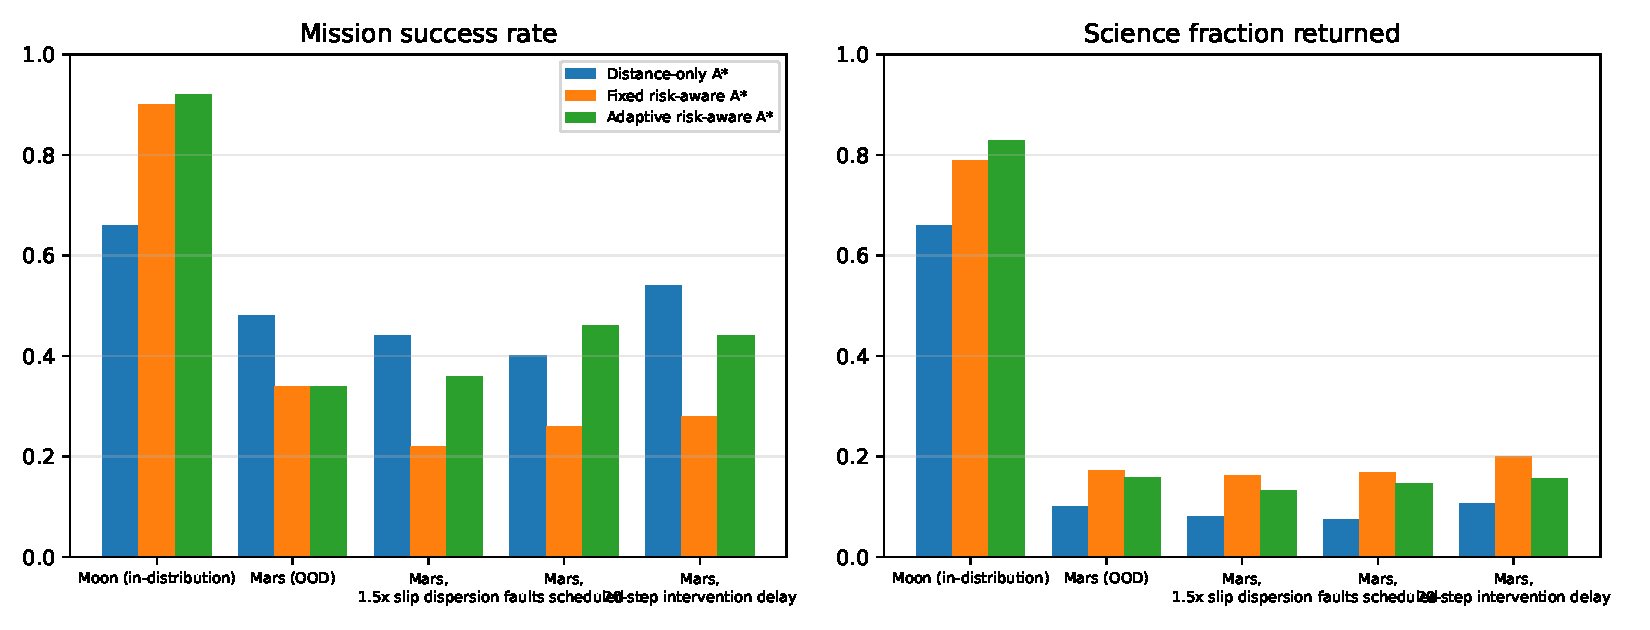
\includegraphics[width=\textwidth]{figures/exonaut_main_outcomes.pdf}
\caption{Mission success rate and science fraction by condition and planner.}
\end{figure}

\begin{figure}[htbp]
\centering
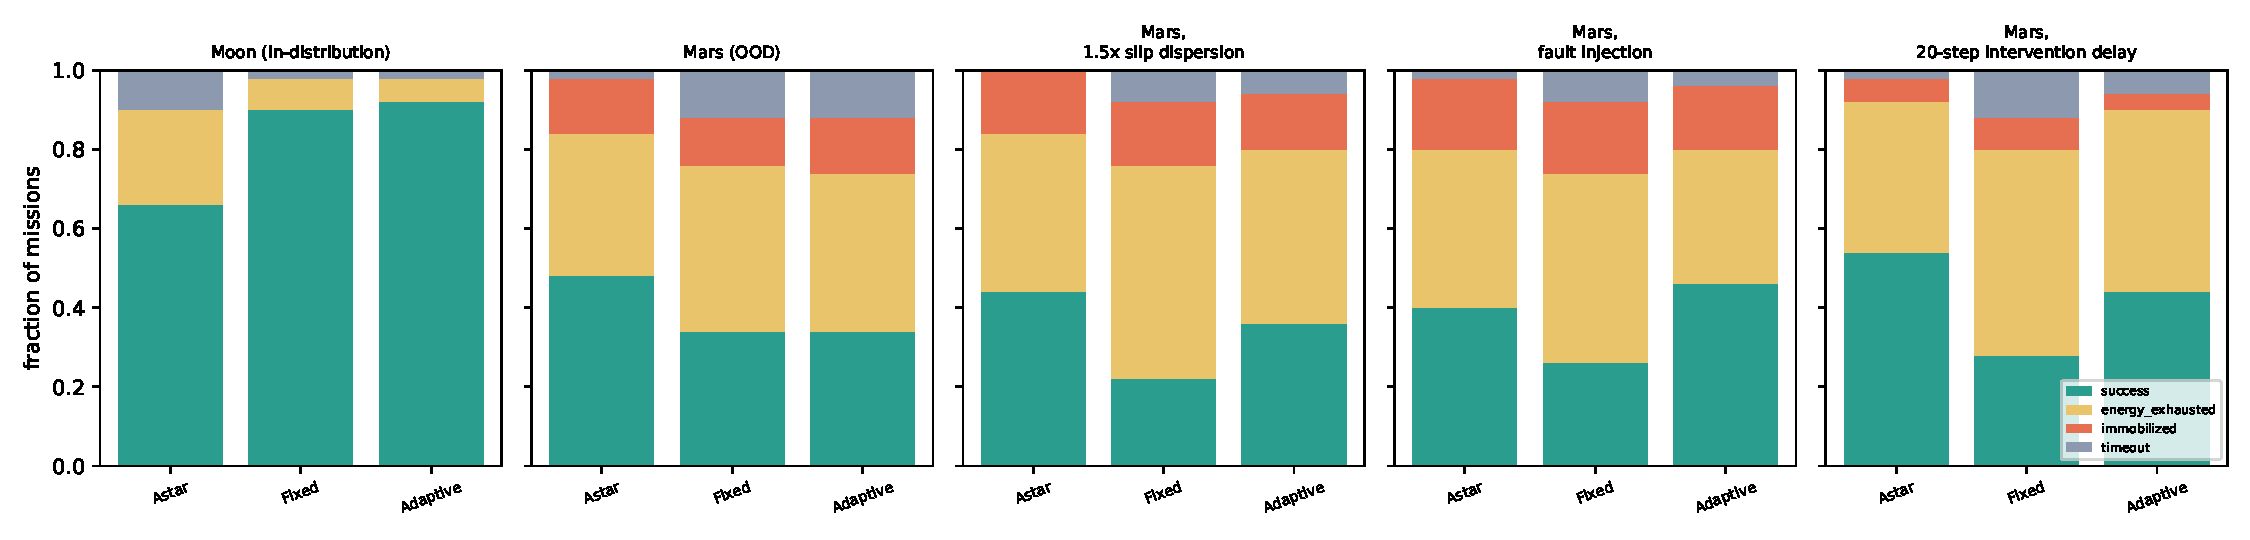
\includegraphics[width=\textwidth]{figures/exonaut_main_terminations.pdf}
\caption{How missions ended. Descriptively, the adaptive planner ends fewer
missions in energy exhaustion than the fixed planner in every condition. This
was not a pre-specified test.}
\end{figure}

\section{After Study 1: simulator audit and methodological corrections}
\label{sec:audit}

Everything in this section was found or done after Study~1's results were
seen. None of it changes Study~1's reported numbers; it changes how some of
them should be read, and it shapes Study~2.

\subsection{Defects and their effect on Study 1}

Table~\ref{tab:defects} lists the defects found. Each is fixed in engine
profile \emph{v2}, which is selected explicitly; v1 remains the default and
still reproduces every Study~1 mission.

\begin{table}[h]
\centering\small
\begin{tabular}{p{0.28\textwidth}p{0.36\textwidth}p{0.26\textwidth}}
\toprule
Defect in v1 & Effect on Study 1 & Fix in v2 \\
\midrule
Learner treats each slip reading as a near-exact measurement of the class mean &
beliefs overconfident (coverage \AuditCoverageCommitted{}) & per-reading variance includes class dispersion \\
Faults drawn over the whole horizon & ``faults'' condition mostly fault-free (H3 not a fault effect) & faults inside the mission \\
One random stream for every purpose & cross-condition comparisons change all noise & separate streams \\
Hazard-threshold relaxation never reset & hazard avoidance relaxed after early help requests & one planning cycle only \\
Livelock at the lander & most timeouts are parked rovers & recharge and reconsider \\
Reported minimum charge can miss the final draw & descriptive \texttt{min\_charge} slightly high & final state included \\
\bottomrule
\end{tabular}
\caption{Defects found after Study~1. Details and counts:
\texttt{docs/RESEARCH\_LOG.md}.}
\label{tab:defects}
\end{table}

An exploration of v2 on validation seeds only (\texttt{docs/EXPLORATION\_V2.md},
generated from its data) found that the fixes do what they claim, and that with
them in place adaptation's survival advantage on validation seeds largely
disappears. It also showed that the communication-delay condition has no
mechanism under v2, since delay acts only through help requests and v2 almost
never asks for help; Study~2 drops it.

A simulator validation suite now checks terrain, motion, energy accounting,
slip sampling, fault timing and streams, planner equivalence, absence of
ground-truth access by any planner, and the single enforcement point of the
risk budget (\texttt{docs/SIMULATOR\_VALIDATION.md}). It must pass before
Study~2 may run.

\subsection{Calibration audit of the terrain learner}

Because the planner turns its slip uncertainty into P(fail), the learner's
intervals must mean what they say. On train seeds, the v2 learner's nominal
95\% interval for a class's mean slip contained the truth
\CalDiagBaseMarsCovNinetyFive{} of the time on Mars and
\CalDiagBaseMoonCovNinetyFive{} on the Moon --- miscalibrated even in
distribution. Diagnostic ablations using simulator truth attributed most of
this to misclassification: \CalMisclassShareMars\% (Mars) and
\CalMisclassShareMoon\% (Moon) of slip readings were filed under the wrong
terrain class, and filing them under the true class alone raised coverage to
\CalDiagNoMisclassMarsCovNinetyFive{} (Mars) and
\CalDiagNoMisclassMoonCovNinetyFive{} (Moon). The rest of the Martian shortfall
is the lunar prior's conflict with Martian loose fines --- the domain shift itself.

Six candidate corrections, their fitting data (train seeds only) and an
acceptance rule were fixed before any validation run
(\texttt{docs/CALIBRATION\_AUDIT.md}). The candidates were: no change; a
confusion-aware learner that shares each reading among the classes that could
have produced it, using the rover's own classifier error rate (no fitted
parameter); a conformal scale on the reported uncertainty, fit on lunar or on
Martian training missions; and the two combined. The rule required, on Mars,
95\% coverage in $[0.90, 0.99]$ and 50, 80 and 90\% coverage each within 0.10 of
nominal, and on the Moon 95\% coverage of at least 0.90.

\textbf{No candidate met the rule} (Figure~\ref{fig:calibration}). The
confusion-aware learner was calibrated on the Moon at every level (95\%:
\CalMThreeMoonCovNinetyFive{}) but reached only \CalMThreeMarsCovNinetyFive{}
on Mars, where the lunar prior's error on loose fines remains (fines coverage
\CalMThreeMarsFinesCov{}). The closest scaled candidate, a scale of
\CalScaleMTwoMoon{} fit on lunar missions, reached \CalMTwoAMarsCovNinetyFive{}
at the 95\% level on Mars but over-covered at 50\%
(\CalMTwoAMarsCovFifty{}), because one scale cannot fit a residual distribution
in which most beliefs are accurate and a few are far off. The rule was not
changed after the result was seen; choosing how to proceed is recorded as an
open decision for Study~2.

\begin{figure}[t]
\centering
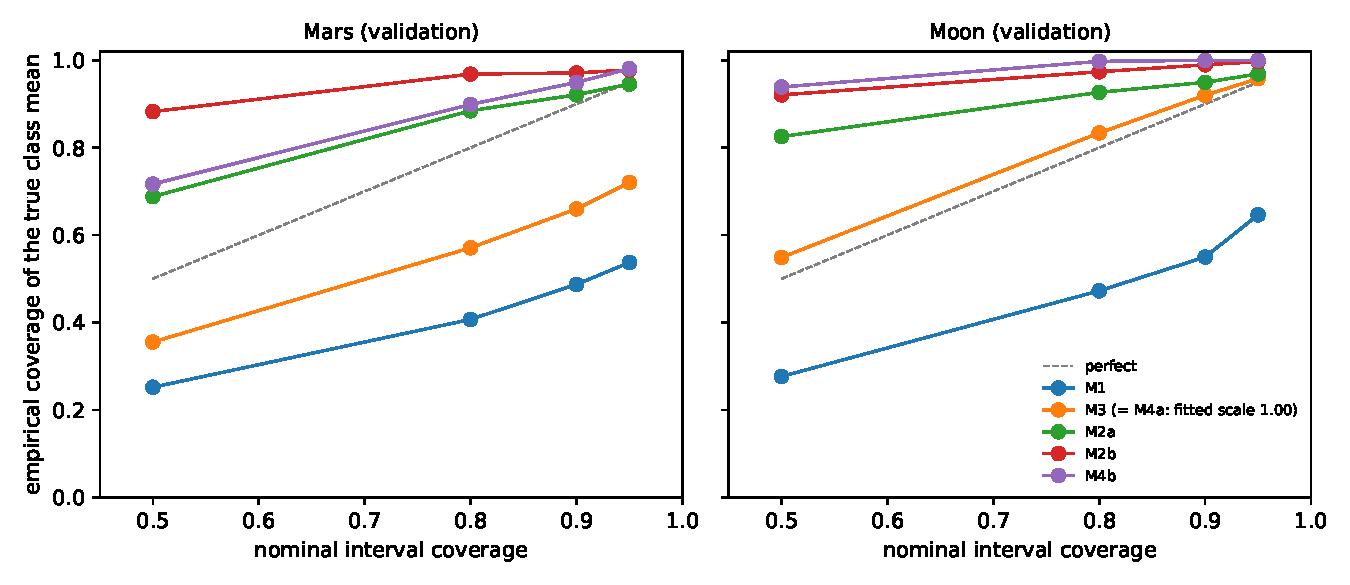
\includegraphics[width=\textwidth]{figures/v2_calibration_curve.pdf}
\caption{Empirical versus nominal coverage of the class-mean intervals on
validation seeds, for each pre-specified calibration candidate. The dashed
line is perfect calibration. Development data only; not a confirmatory
result.}
\label{fig:calibration}
\end{figure}

\section{Study 2: planned, not executed}
\label{sec:study2}

Study~2 has not been run, and this section reports no result. Its purpose is a
narrower, cleaner test of one question:

\begin{quote}
Does online adaptation of terrain slip beliefs improve safe mission completion
under terrain-model shift, compared with an otherwise identical fixed
risk-aware planner, and what does it cost in science return?
\end{quote}

\paragraph{Design (draft).} The fixed and adaptive planners differ only in
whether measured slip revises the class beliefs; both use the v2 engine, the
same lunar prior and the same calibration settings. The confirmatory condition
is Mars with a lunar prior. The Moon condition is secondary; higher dispersion
and faults are exploratory; communication delay is dropped (above).

\paragraph{Outcomes and hypotheses (draft).} Primary: mission success in the
Mars condition, tested two-sided with McNemar's exact test at $\alpha =
\PowAlpha$ on matched seeds. No direction is hypothesised: Study~1 found an
exact tie in Martian success and the validation exploration found differences
whose intervals touched zero. Secondary: science fraction on Mars (two-sided
paired $t$), and success and science fraction on the Moon, Holm-corrected as a
family. Everything else is descriptive or exploratory
(\texttt{docs/V2\_HYPOTHESES\_DRAFT.md}).

\paragraph{Sample size.} The power of McNemar's test depends on the effect to
detect and on how often the two planners disagree (the discordance rate). The
minimum effect of interest is fixed at $\PowMinEffect$ in success probability.
The discordance rate was estimated on \PowMThreeValSeeds{} validation seeds per
body for each of the two leading calibration candidates, and its one-sided
90\% upper bound was used. The estimated effect itself was deliberately not
used to size the study. Exact power calculations give, for power
$\PowTarget$, \PowMThreeRecommendedN{} matched seeds with the confusion-aware
learner and \PowMTwoARecommendedN{} with the scaled learner
(Figure~\ref{fig:power}; \texttt{docs/POWER\_ANALYSIS.md}).

\begin{figure}[t]
\centering
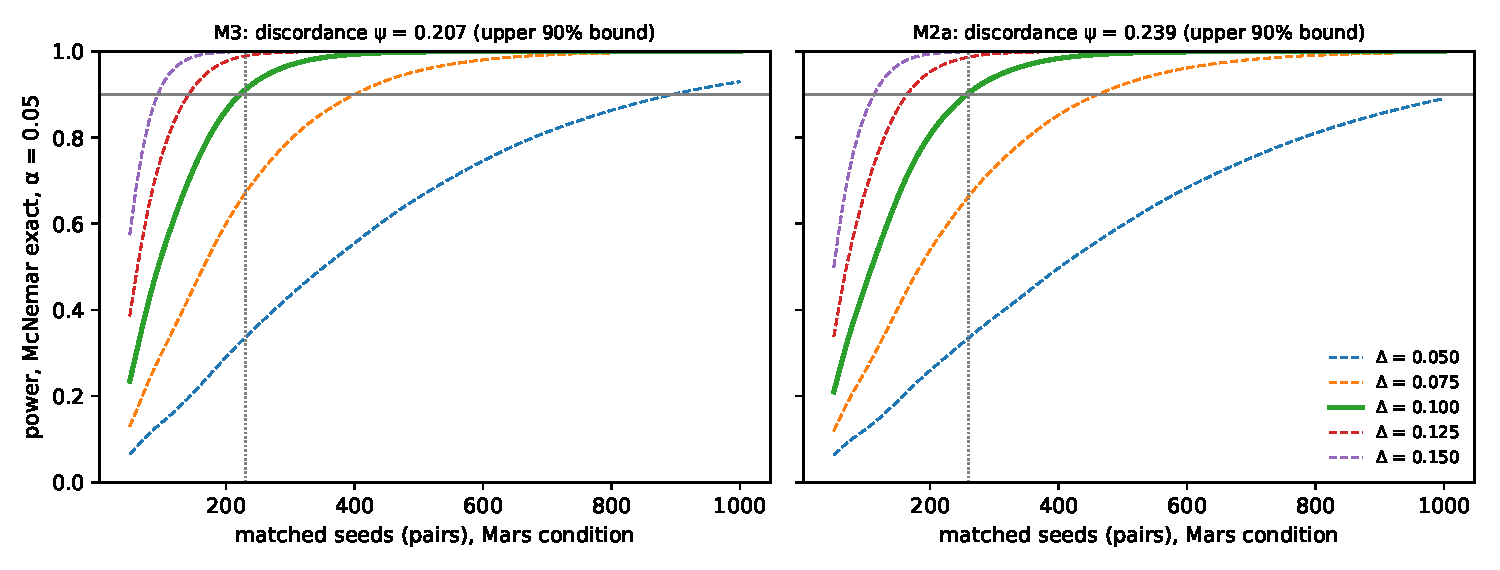
\includegraphics[width=\textwidth]{figures/v2_power_curve.pdf}
\caption{Exact power of the planned primary test against the number of matched
seeds, for several effect sizes (solid: the minimum effect of interest), at the
upper-bound discordance rate estimated on validation seeds for each leading
calibration candidate. Planning quantities only.}
\label{fig:power}
\end{figure}

\paragraph{Seeds and access control.} Study~2's confirmatory seeds are new: two
pools of \PowPool{} drawn from a range disjoint from every Study~1 split, by a
recorded algorithm and master seed. The terrain generator refuses them unless
the frozen analysis plan exists and the run is authorised with that plan's
hash, and it logs every attempt. At the time of writing no Study~2
confirmatory terrain has been generated.

\paragraph{What must happen before it runs.} A freeze checklist
(\texttt{docs/V2\_FREEZE\_CHECKLIST.md}) requires, among other items, an
accepted calibration method, a passing simulator validation suite, frozen
hypotheses, tests, multiplicity plan and sample size, and a clean access log.
It is currently blocked on calibration.

\section{Discussion}

The result we set out to find is not the result we obtained. H2, the
hypothesis that online adaptation would raise science return under domain
shift, is not supported: the effect was absent on held-out seeds despite
appearing clearly during tuning. The one contrast that survived correction
turned out, on audit, not to measure what its condition was named for, so H3 is
not supported either. What remains is a descriptive pattern in which adaptation
trades a little science for survival. It is consistent with a plausible
mechanism, but it was not tested as such, and it comes from a learner now known
to be miscalibrated.

Three things follow.

First, the interesting version of this experiment has not been run yet.
Study~2 is designed to be that version, and preparing it has already produced a
finding of its own: the learner at the centre of the adaptive planner was
miscalibrated even on familiar terrain, mostly through terrain
misclassification, and while that can be fixed without fitting anything, no
simple correction calibrated it under the domain shift itself. A risk-aware
planner inherits whatever its uncertainty model gets wrong, so this is not a
side issue for Study~2.

Second, caution has a price that risk-aware formulations do not currently
charge. On terrain where most ground is hazardous, detouring is not free, and
the uninformed planner's survival advantage came from simply spending less
time exposed. A more complete objective would price route length and exposure
time against per-cell risk rather than treating risk avoidance as costless.

Third, the gap between the validation and confirmatory estimates is the most
methodologically useful outcome here. A tuning-set advantage of $+0.125$ to
$+0.167$ in Martian success became $0.000$ on held-out seeds. Had the seed
protocol not been frozen in advance, that first number is the one that would
have been reported.

\subsection{Future work}

The obvious extensions are to adapt the locomotion multiplier as well as the
slip model, to add exposure time to the planner's objective so that caution is
priced, and to test transfer in the reverse direction (Mars prior, lunar
deployment) to check that the effects here are not specific to one direction of
shift.

\section{Limitations}
\label{sec:limitations}

Stated plainly, because the value of this study depends on what it does not
claim.

\begin{enumerate}[leftmargin=2em]
  \item \textbf{This is not a validated rover model.} Terrain parameters were
  chosen to produce the qualitative regimes the experiment needs --- a
  low-traction trap, a high-traction refuge, impassable rims, and true
  darkness --- and are not calibrated against measured lunar or Martian
  geotechnical data. Absolute values are properties of this simulator.
  \item \textbf{2.5-D, not dynamics.} There is no vehicle suspension, no wheel
  contact mechanics, and no attitude. Slip is drawn from a distribution rather
  than emerging from terramechanics.
  \item \textbf{Risk composition is approximate.} Equations~\ref{eq:embed} and
  \ref{eq:risk} treat per-cell events as independent, which understates risk in
  homogeneous terrain. It is applied identically to all planners.
  \item \textbf{Only the slip model adapts.} The per-class locomotion
  multiplier is not revised online. Energy estimates still improve through the
  slip channel, since slip enters Equation~\ref{eq:energy} directly, but a
  systematic error in $m_k$ would persist.
  \item \textbf{The analysis plan is not a true pre-registration.} It was
  written after the adaptive planner existed and after an eight-seed
  engineering pilot had been seen. Those eight seeds are quarantined, and the
  full timeline is recorded in \texttt{docs/RESEARCH\_LOG.md}.
  \item \textbf{Two bodies, one prior direction.} Only Moon$\rightarrow$Mars
  transfer is tested. The reverse direction, and bodies beyond these two, are
  untested.
  \item \textbf{The adaptive learner is overconfident.} The conjugate update
  (Equation~\ref{eq:conjugate}) uses an observation variance of $0.02^2$ per
  slip reading. That treats a reading as a near-exact measurement of the class
  mean, when readings actually scatter by the terrain's own dispersion
  (standard deviation 0.04--0.18). One reading therefore moves the belief most
  of the way to itself, and the reported uncertainty is far too small (95\%
  coverage \AuditCoverageCommitted{}; see Results). All confirmatory results use
  this rule.
  \item \textbf{Faults mostly did not fire.} Fault times are drawn over the whole
  \AuditHorizon-step horizon, but missions end much sooner, so the ``hardware
  faults'' condition exposed only \AuditFiredAdaptive{}--\AuditFiredFixed{} of
  missions to any fault. It is not a test of fault tolerance.
  \item \textbf{One random stream serves every purpose.} Terrain, layout, fault
  schedule and every slip draw come from one generator in sequence. With no
  faults configured, the fault draw is skipped, so every later slip draw shifts.
  Paired contrasts within a condition are unaffected, because both planners in a
  pair share a stream. Comparisons across conditions, however, change the whole
  noise realisation, not just the named factor.
  \item \textbf{Intervention relaxation ratchets.} Each ground intervention
  raises the planner's hazard threshold by 0.15, up to 0.95, and it is never
  restored. Martian missions requested many interventions, so in most of them
  the planners' hazard avoidance was effectively relaxed early. This applies to
  every planner equally.
  \item \textbf{Most timeouts are a livelock at the lander.} When the rover is
  home and no target fits the risk budget, the mission logic neither writes the
  remaining targets off nor stops. It keeps requesting interventions until the
  step limit, so most ``timeout'' failures are rovers parked safely at the
  lander. Planners reach this state at different rates, so it affects the
  success comparison; the counts are in \texttt{docs/RESEARCH\_LOG.md}.
  \item \textbf{The five items above, from the learner's overconfidence to the
  livelock, are Study~1 defects,} fixed in engine profile v2
  (Section~\ref{sec:audit}); Study~1's numbers are reported as run.
  \item \textbf{Calibration under shift is unsolved.} On development data no
  pre-specified correction calibrated the learner on Mars at every level
  (Section~\ref{sec:audit}).
  \item \textbf{Idealisations in the learner.} It removes the slope's effect on a
  reading using the true slope of the cell driven, standing in for a
  noise-free attitude sensor; slip is spatially independent between cells.
\end{enumerate}

\section{Reproducibility}

Every reported number is a macro generated from a committed artifact; no result
value is typed into this document. \texttt{paper/PROVENANCE.yaml} records, for
every generated table, figure and macro, the script that produced it, its hash,
its input files and their hashes, and the commit; a test fails if any of them
is stale or edited by hand, and continuous integration re-runs every
generator. The run's metadata sidecar records the git commit, the seed-split
checksum, the quarantine list and library versions. The pipeline is:

\begin{verbatim}
python scripts/freeze_seed_protocol.py        # once; refuses to overwrite
python scripts/calibrate_priors.py            # priors from TRAIN seeds only
python scripts/run_exonaut_experiments.py     # Study 1 confirmatory sweep
python scripts/verify_v1_reproduction.py      # all 750 Study 1 missions
python scripts/calibration_study.py diagnose  # then fit, evaluate, report
python scripts/power_analysis.py run          # then analyze
python scripts/build_all_figures.py           # every figure, table, macro
\end{verbatim}

\bibliographystyle{plain}
\bibliography{references}

\end{document}
